\documentclass[11pt,a4paper]{article}
\usepackage[left=2cm,top=3cm,text={17cm,24cm}]{geometry}
\usepackage[utf8]{inputenc}
\usepackage[czech]{babel}
\usepackage{blindtext}
\usepackage[unicode,pdfpagelabels]{hyperref}
\usepackage{multirow}
\usepackage{csquotes}
\usepackage[czech,linesnumbered,ruled,noline,longend]{algorithm2e}
\usepackage{graphicx}
\usepackage{pdflscape}

\hbadness=999999
\pdfoptionpdfminorversion=7

\begin{document}

\hypersetup{pageanchor=false}
\begin{titlepage}
    \begin{center}
    \Huge\textsc{Vysoké učení technické v~Brně}\\
    \huge\textsc{Fakulta informačních technologií}\\
    \renewcommand{\baselinestretch}{0.4}
    \vspace{\stretch{0.382}}
    \LARGE{Typografie a~publikování\,--\,3.~projekt}\\
    \vspace{0.5em}
    \Huge{Tabulky a~obrázky}\\
    \vspace{\stretch{0.618}}
    \renewcommand{\baselinestretch}{0.3}
    \end{center}
\Large {1. duben 2019 \hfill Peter Koprda}
\end{titlepage}
\hypersetup{pageanchor=true}

\newpage

\section{Úvodní strana}
    Název práce umístěte do~zlatého řezu a~nezapomeňte uvést dnešní datum a~vaše jméno a~příjmení.


\section{Tabulky}
    Pro~sázení tabulek můžeme použít buď prostředí\texttt{ tabbing }nebo prostředí\texttt{ tabular}.

    \subsection{Prostředí \texttt{tabbing}}
        Při použití \texttt{tabbing} vypadá tabulka následovně:

        \begin{tabbing}
		    Vodní melouny \quad	\= \textbf{Cena} \quad	\= \textbf{Množství}\kill
		    \textbf{Ovoce}		\> \textbf{Cena}		\> \textbf{Množství}\\
		    Jablka				\> 25,90				\> 3 kg\\
		    Hrušky				\> 27,40				\> 2,5 kg\\
		    Vodní melouny		\> 35,--				\> 1 kus\\
        \end{tabbing}
        Toto prostředí se dá také použít pro sázení algoritmů, ovšem vhodnější je použít prostředí \texttt{algorithm} nebo \texttt{algorithm2e} (viz sekce~\ref{section:algoritmy}).

    \subsection{Prostředí \texttt{tabular}}
        Další možností, jak vytvořit tabulku, je použít prostředí \texttt{tabular}. Tabulky pak budou vypadat takto\footnotemark:

        \catcode`\-=12
        \bigskip
        \begin{table}[h]
            \centering
            \begin{tabular}{|c|c|c|l}
                \cline{1-3}
                \multirow{2}{*}     & \multicolumn{2}{c |}{\textbf{Cena}}	\\
                \cline{2-3}
			    \textbf{Měna}	    & \textbf{nákup}	          & \textbf{prodej}   \\
                \cline{1-3}
                EUR                 & 25,615                      & 27,20           &   \\
                GBP                 & 29,899                      & 31,80           &   \\
                USD                 & 22,571                      & 25,51           &   \\
                \cline{1-3}
            \end{tabular}
            \caption{Tabulka kurzů k~dnešnímu dni}
            \label{table:kurzy}
        \end{table}
        \bigskip

        \begin{table}[h]
            \centering
            \begin{tabular}[p]{|c|c|cl}
                \hline
                A               & $\neg{A}$  \\ \hline
                \textbf{P}      & N       \\ \hline
                \textbf{O}      & O       \\ \hline
                \textbf{X}      & X       \\ \hline
                \textbf{N}      & P       \\ \hline
            \end{tabular}
            \begin{tabular}[p]{|c|c|c|c|c|c|}
                \hline
                \multicolumn{2}{|l|}{\multirow{2}{*}{$A \wedge B$ }} & \multicolumn{4}{c|}{B}               \\
                \cline{3-6}
                \multicolumn{2}{|l|}{}                  & \textbf{P} & \textbf{O} & \textbf{X} & \textbf{N}  \\
                \cline{1-2}\cline{3-6}
                \multirow{4}{*}{A} & \textbf{P}         & P          & O          & X          & N           \\
                \cline{2-6}
                                   & \textbf{O}         & O          & O          & N          & N           \\
                \cline{2-6}
                                   & \textbf{X}         & X          & N          & X          & N           \\
                \cline{2-6}
                                   & \textbf{N}         & N          & N          & N          & N           \\
                \hline
            \end{tabular}
            \begin{tabular}[p]{|c|c|c|c|c|c|}
                \hline
                \multicolumn{2}{|l|}{\multirow{2}{*}{$A \vee B$ }} & \multicolumn{4}{c|}{B}                             \\
                \cline{3-6}
                \multicolumn{2}{|l|}{}                             & \textbf{P} & \textbf{O} & \textbf{X} & \textbf{N}  \\
                \hline
                \multirow{4}{*}{A} & \textbf{P}                    & P          & P          & P          & P           \\
                \cline{2-6}
                                   & \textbf{O}                    & P          & O          & P          & O           \\
                \cline{2-6}
                                   & \textbf{X}                    & P          & P          & X          & X           \\
                \cline{2-6}
                                   & \textbf{N}                    & P          & O          & X          & N           \\
                \hline
            \end{tabular}
            \begin{tabular}[p]{|c|c|c|c|c|c|}
                \hline
                \multicolumn{2}{|l|}{\multirow{2}{*}{$A \rightarrow B$ }} & \multicolumn{4}{c|}{B}                             \\
                \cline{3-6}
                \multicolumn{2}{|l|}{}                                         & \textbf{P} & \textbf{O} & \textbf{X} & \textbf{N}  \\
                \hline
                \multirow{4}{*}{A} & \textbf{P}                                & P          & O          & X          & N           \\
                \cline{2-6}
                                   & \textbf{O}                                & P          & O          & P          & O           \\
                \cline{2-6}
                                   & \textbf{X}                                & P          & P          & X          & X           \\
                \cline{2-6}
                                   & \textbf{N}                                & P          & P          & P          & P           \\
                \hline
            \end{tabular}
            \caption{Protože Kleeneho trojhodnotová logika už je \enquote{zastaralá}, uvádíme si zde příklad čtyřhodnotové logiky}
            \label{table:logika}
        \end{table}

        \footnotetext{Kdyby byl problém s~\texttt{cline}, zkuste se podívat třeba sem:
        \url{http://www.abclinuxu.cz/tex/poradna/show/325037}.}

        \pagebreak


\newpage

\section{Algoritmy}
    \label{section:algoritmy}
    Pokud budeme chtít vysázet algoritmus, můžeme použít prostředí \texttt{algorithm}\footnotemark
    \footnotetext{Pro nápovědu, jak zacházet s~prostředím \texttt{algorithm}, můžeme zkusit tuhle stránku:\\
    \url{http://ftp.cstug.cz/pub/tex/CTAN/macros/latex/contrib/algorithms/algorithms.pdf}.}
    nebo \texttt{algorithm2e}\footnotemark.
    Příklad použití prostředí \texttt{algorithm2e} viz Algoritmus~\ref{algorithm:1}.\\

    \footnotetext{Pro \texttt{algorithm2e} zase tuhle:
    \url{http://ftp.cstug.cz/pub/tex/CTAN/macros/latex/contrib/algorithm2e/algorithm2e.pdf}.}

    \IncMargin{1.5em}
    \begin{algorithm}
        \label{algorithm:1}
        \DontPrintSemicolon
        \SetNlSty{}{}{:}
        \SetNlSkip{0.4em}
        \SetAlgoNlRelativeSize{-1}
		\SetInd{1em}{1em}
		\SetKwInput{Output}{Output}
        \SetKwInput{Input}{Input}

		\Indm\Indmm
        \Input{~($X_{t-1},u_t,z_t$)}
        \Output{~$X_t$}
        \Indp\Indpp
        \BlankLine
        $ \overline{X_t} = X_t = 0$\;
        \For{$k=1 \textrm{\emph{ to }} M $}
        {
            $x^{[k]}=\emph{sample\_motion\_model}(u_t,x^{[k]}_{t-1})$\;
            $\omega^{[k]}_t=\emph{measurement\_model}(z_t,x^{[k]}_t,m_{t-1})$\;
            $m^{[k]}_t=\emph{update\_occupancy\_grid}(z_t,x^{[k]}_t,m^{[k]}_{t-1})$\;
            $\overline{X_t}=\overline{X_t}+\langle x^{|m|}_x,\omega^{|m|}_t\rangle$\;
        }
        \For{$k=1 \textrm{\emph{ to }} M $}
        {
            draw \emph{i} with probability $\approx \omega^{[i]}_t$\;
            add $\langle x^{[k]}_x,m^{[k]}_t \rangle$ to $X_t$\;
        }
        \KwRet${X_t}$
        \caption{\textsc{FastSLAM}}
    \end{algorithm}
    \DecMargin{1.5em}


\section{Obrázky}
    Do~našich článků můžeme samozřejmě vkládat obrázky. Pokud je obrázkem fotografie,
    můžeme klidně použít bitmapový soubor. Pokud by to ale mělo být nějaké schéma nebo
    něco podobného, je dobrým zvykem takovýto obrázek vytvořit vektorově.\\
    \begin{figure}[htb]
        \centering
        \scalebox{0.35}
        {
            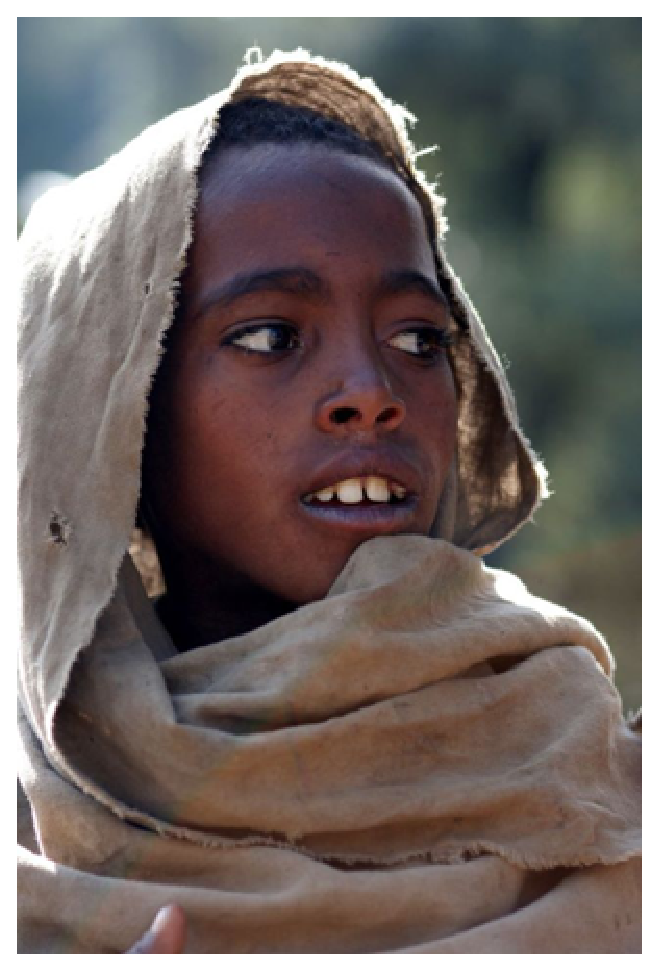
\includegraphics{etiopan.eps}
            \reflectbox{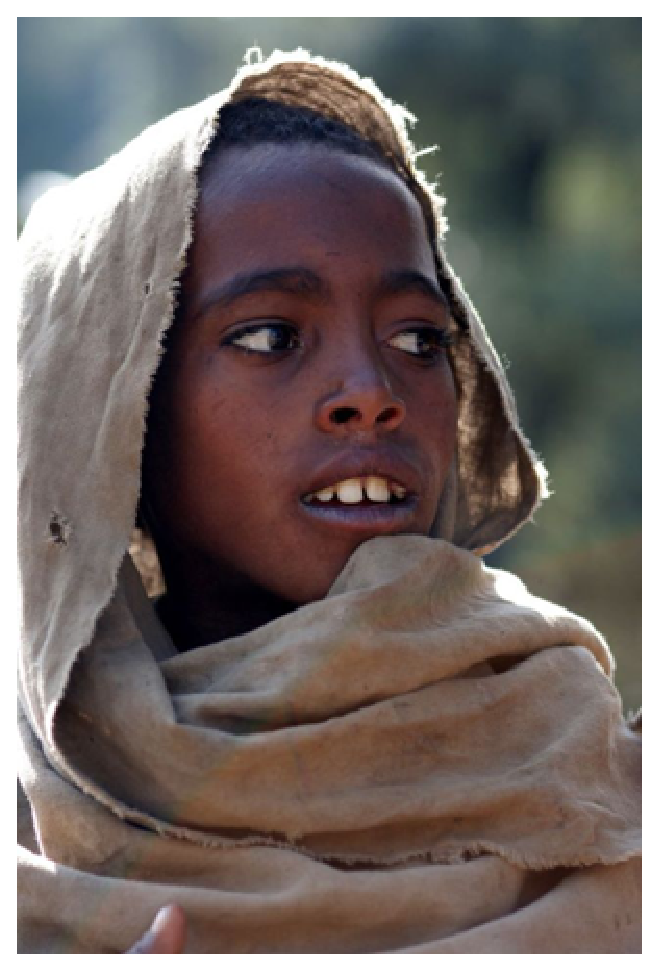
\includegraphics{etiopan}}
        }
        \caption{Malý Etiópanek a~jeho bratříček}
        \label{figure:etiopan}
    \end{figure}

    \pagebreak
    \newpage
    Rozdíl medzi vektorovým\,\dots
    \begin{figure}[htb]
        \centering
        
\includegraphics[scale=0.4]{oniisan}
        \caption{Vektorový obrázek}
        \label{figure:vektor}
    \end{figure}

    \bigskip
    \noindent\,\dots a~bitmapovým obrázkem
    \begin{figure}[tbh]
        \centering
        
\includegraphics[scale=0.6]{oniisan2}
        \caption{Bitmapový obrázek}
        \label{figure:bitmap}
    \end{figure}

    \bigskip
    \noindent se projeví například při zvětšení.\par
    Odkazy (nejen ty) na~obrázky~\ref{figure:etiopan}, ~\ref{figure:vektor} a~\ref{figure:bitmap}, na~tabulky~\ref{table:kurzy} a~\ref{table:logika}~a také na algoritmus~\ref{algorithm:1} jsou udělány pomocí křížových odkazů. Pak je ovšem potřeba zdrojový soubor přeložit dvakrát.\par
    Vektorové obrázky lze vytvořit i~přímo v~{\LaTeX}u, například pomocí prostředí \texttt{picture}.

\pagebreak

\begin{landscape}
    \begin{figure}[ht]
        \setlength{\unitlength}{1mm}
        \begin{picture}(220,130)
            \linethickness{1pt}
            \put(20, 0){\framebox(220, 130){}}

            \linethickness{1.5mm}
    		\put(24,14){\line(1,0){210}}
    		
    		\linethickness{1pt}
    		
            %%%%% HOUSE %%%%%
            \put(40,14){\line(0,1){40}}
            \put(48,14){\line(0,1){30}}
            \put(40,54){\line(1,0){30}}
            \put(70,50){\line(0,1){40}}
            \put(72,70){\line(1,0){28}}
            \put(72,80){\line(1,0){28}}
            \put(72,70){\line(0,1){10}}
            \put(100,70){\line(0,1){10}}
            \put(110,70){\line(1,0){15}}
            \put(110,70){\line(0,1){8}}
            \put(110,78){\line(1,0){15}}
            \put(125,70){\line(0,1){8}}
            \put(70,50){\line(1,0){20}}
            \put(90,50){\line(0,1){10}}
            \put(90,60){\line(1,0){60}}
            \put(150,14){\line(0,1){46}}
            \put(90,50){\line(1,0){50}}
            \put(105,60){\line(0,1){30}}
            \put(147,68){\line(1,0){20}}
            \put(147,86){\line(1,0){20}}
            \put(147,68){\line(0,1){18}}
            \put(167,68){\line(0,1){18}}
            \put(150,68){\line(0,1){18}}
            \put(151,68){\line(0,1){18}}
            \put(162,68){\line(0,1){18}}
            \put(163,68){\line(0,1){18}}
            \put(70,90){\line(1,0){35}}
            \put(105,90){\line(1,0){25}}
            \put(130,90){\line(-1,6){4}}
            \put(130,90){\line(0,-1){30}}
            \put(125,115){\line(5,-2){45}}
            \put(145,97){\line(1,0){25}}
            \put(145,97){\line(0,-1){37}}
            \put(150,55){\line(1,0){20}}
            \put(170,55){\line(0,1){42}}
            \put(170,60){\line(1,0){35}}
            \put(205,60){\line(0,-1){45}}
            \put(195,14){\line(0,1){35}}
            \put(195,49){\line(-1,0){40}}
            \put(155,49){\line(0,-1){36}}
            \put(140,14){\line(0,1){36}}
            \put(48,44){\line(1,0){40}}
            \put(88,14){\line(0,1){30}}
            \put(93,14){\line(0,1){48}}
            \put(94,14){\line(0,1){48}}
            \put(96,14){\line(0,1){48}}
            \put(97,14){\line(0,1){48}}
            \put(99,14){\line(0,1){48}}
            \put(100,14){\line(0,1){48}}
            \put(102,14){\line(0,1){36}}
            \put(104,14){\line(0,1){28}}
            \put(104,42){\line(1,0){10}}
    		\put(114,14){\line(0,1){28}}
            \put(120,25){\line(0,1){20}}
            \put(120,45){\line(1,0){10}}
            \put(130,25){\line(0,1){20}}
            \put(120,25){\line(1,0){10}}
            
    		%%%%% SUN %%%%%
    		\put(220, 115){\circle{14}}
    		
        \end{picture}
        \caption{Vektorový obrázek domu}
    \end{figure}
\end{landscape}


\end{document} 